\documentclass{standalone}
\usepackage{tikz}
\usetikzlibrary{patterns, positioning}


\begin{document}
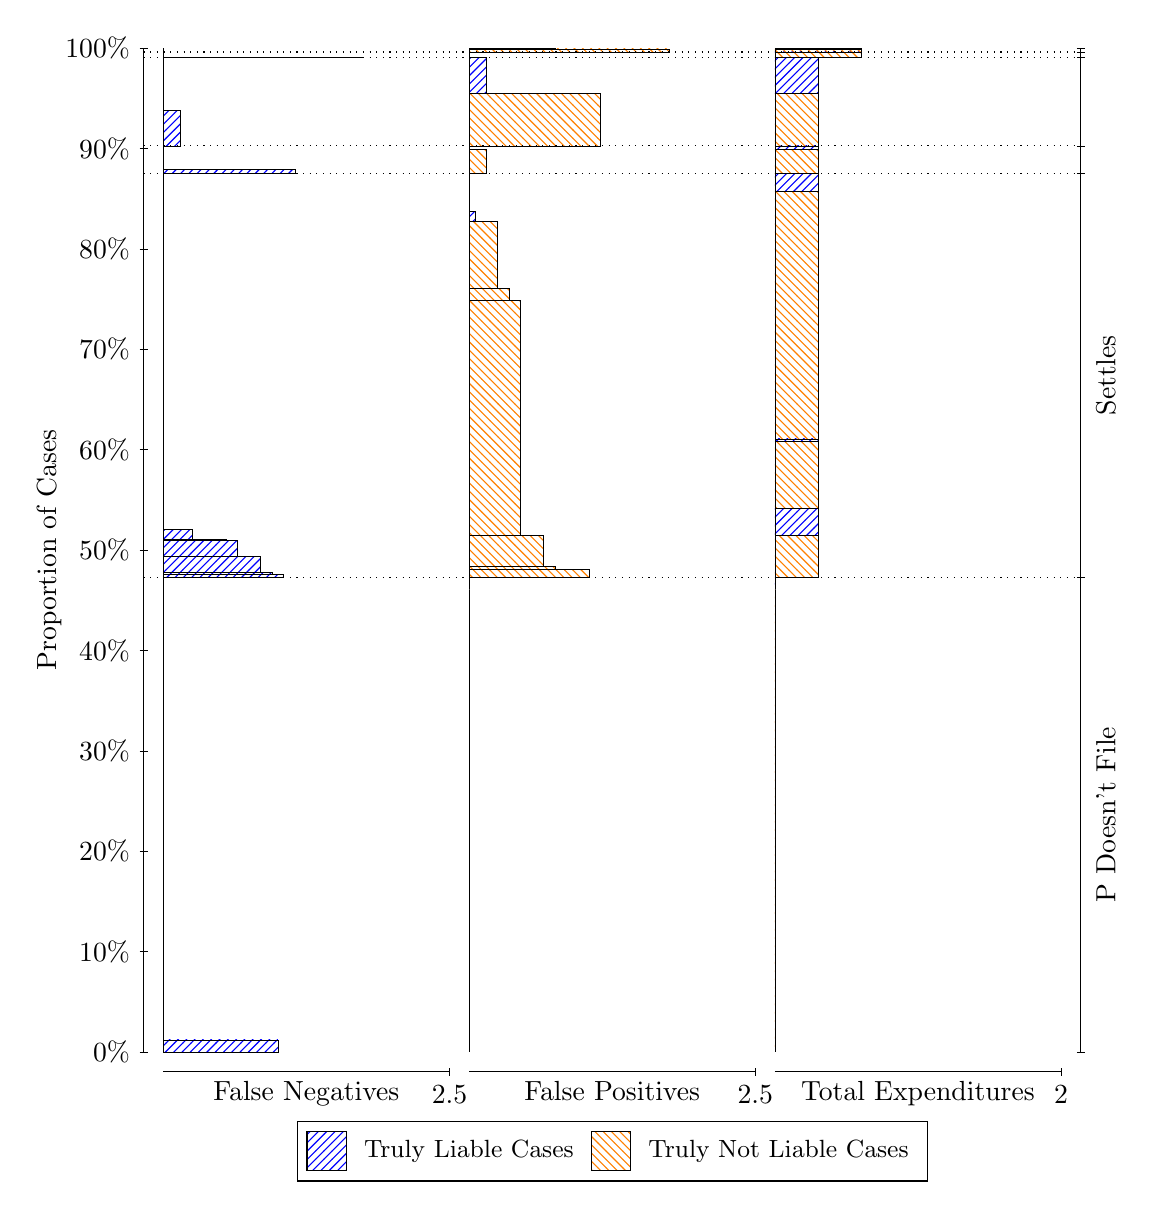
\begin{tikzpicture}
\draw[black, very thin] (1.5,1.75) -- (1.5,14.5);
\node[rotate=90, text=black, anchor=center] at (0.3, 8.125) {Proportion of Cases};
\draw[black, very thin] (1.45,1.75) -- (1.55,1.75);
\node[text=black, anchor=east] at (1.45, 1.75) {0\%};
\draw[black, very thin] (1.45,3.025) -- (1.55,3.025);
\node[text=black, anchor=east] at (1.45, 3.025) {10\%};
\draw[black, very thin] (1.45,4.3) -- (1.55,4.3);
\node[text=black, anchor=east] at (1.45, 4.3) {20\%};
\draw[black, very thin] (1.45,5.575) -- (1.55,5.575);
\node[text=black, anchor=east] at (1.45, 5.575) {30\%};
\draw[black, very thin] (1.45,6.85) -- (1.55,6.85);
\node[text=black, anchor=east] at (1.45, 6.85) {40\%};
\draw[black, very thin] (1.45,8.125) -- (1.55,8.125);
\node[text=black, anchor=east] at (1.45, 8.125) {50\%};
\draw[black, very thin] (1.45,9.4) -- (1.55,9.4);
\node[text=black, anchor=east] at (1.45, 9.4) {60\%};
\draw[black, very thin] (1.45,10.675) -- (1.55,10.675);
\node[text=black, anchor=east] at (1.45, 10.675) {70\%};
\draw[black, very thin] (1.45,11.95) -- (1.55,11.95);
\node[text=black, anchor=east] at (1.45, 11.95) {80\%};
\draw[black, very thin] (1.45,13.225) -- (1.55,13.225);
\node[text=black, anchor=east] at (1.45, 13.225) {90\%};
\draw[black, very thin] (1.45,14.5) -- (1.55,14.5);
\node[text=black, anchor=east] at (1.45, 14.5) {100\%};

\draw[black, very thin] (13.4,1.75) -- (13.4,14.5);
\draw[black, very thin] (13.35,1.75) -- (13.45,1.75);
\node[anchor=west] at (13.35, 1.75) {};
\draw[black, very thin] (13.35,7.7786) -- (13.45,7.7786);
\node[anchor=west] at (13.35, 7.7786) {};
\draw[black, very thin] (13.35,12.912) -- (13.45,12.912);
\node[anchor=west] at (13.35, 12.912) {};
\draw[black, very thin] (13.35,13.258) -- (13.45,13.258);
\node[anchor=west] at (13.35, 13.258) {};
\draw[black, very thin] (13.35,14.38) -- (13.45,14.38);
\node[anchor=west] at (13.35, 14.38) {};
\draw[black, very thin] (13.35,14.45) -- (13.45,14.45);
\node[anchor=west] at (13.35, 14.45) {};
\draw[black, very thin] (13.35,14.5) -- (13.45,14.5);
\node[anchor=west] at (13.35, 14.5) {};

\draw[black, very thin, pattern color=blue, pattern=north east lines] (1.75,1.75) rectangle (3.2033,1.9031);
\draw[black, very thin, pattern color=orange, pattern=north west lines] (1.75,1.9031) rectangle (1.75,7.7786);
\draw[black, very thin, pattern color=blue, pattern=north east lines] (1.75,7.7786) rectangle (3.276,7.8126);
\draw[black, very thin, pattern color=blue, pattern=north east lines] (1.75,7.8126) rectangle (3.1307,7.8417);
\draw[black, very thin, pattern color=blue, pattern=north east lines] (1.75,7.8417) rectangle (2.9853,8.0462);
\draw[black, very thin, pattern color=blue, pattern=north east lines] (1.75,8.0462) rectangle (2.6947,8.2422);
\draw[black, very thin, pattern color=blue, pattern=north east lines] (1.75,8.2422) rectangle (2.5493,8.2628);
\draw[black, very thin, pattern color=blue, pattern=north east lines] (1.75,8.2628) rectangle (2.1133,8.3874);
\draw[black, very thin, pattern color=orange, pattern=north west lines] (1.75,8.3874) rectangle (1.75,12.912);
\draw[black, very thin, pattern color=blue, pattern=north east lines] (1.75,12.912) rectangle (3.4213,12.959);
\draw[black, very thin, pattern color=orange, pattern=north west lines] (1.75,12.959) rectangle (1.75,13.258);
\draw[black, very thin, pattern color=blue, pattern=north east lines] (1.75,13.258) rectangle (1.968,13.71);
\draw[black, very thin, pattern color=orange, pattern=north west lines] (1.75,13.71) rectangle (1.75,14.38);
\draw[black, very thin, pattern color=blue, pattern=north east lines] (1.75,14.38) rectangle (4.2933,14.384);
\draw[black, very thin, pattern color=orange, pattern=north west lines] (1.75,14.384) rectangle (1.75,14.45);
\draw[black, very thin, pattern color=orange, pattern=north west lines] (1.75,14.45) rectangle (1.75,14.49);
\draw[black, very thin, pattern color=blue, pattern=north east lines] (1.75,14.49) rectangle (1.75,14.5);
\draw[black, very thin, pattern color=orange, pattern=north west lines] (5.6333,1.75) rectangle (5.6333,7.6255);
\draw[black, very thin, pattern color=blue, pattern=north east lines] (5.6333,7.6255) rectangle (5.6333,7.7786);
\draw[black, very thin, pattern color=orange, pattern=north west lines] (5.6333,7.7786) rectangle (7.1593,7.874);
\draw[black, very thin, pattern color=orange, pattern=north west lines] (5.6333,7.874) rectangle (6.7233,7.9209);
\draw[black, very thin, pattern color=orange, pattern=north west lines] (5.6333,7.9209) rectangle (6.578,8.3101);
\draw[black, very thin, pattern color=orange, pattern=north west lines] (5.6333,8.3101) rectangle (6.2873,11.294);
\draw[black, very thin, pattern color=orange, pattern=north west lines] (5.6333,11.294) rectangle (6.142,11.451);
\draw[black, very thin, pattern color=orange, pattern=north west lines] (5.6333,11.451) rectangle (5.9967,12.303);
\draw[black, very thin, pattern color=blue, pattern=north east lines] (5.6333,12.303) rectangle (5.706,12.428);
\draw[black, very thin, pattern color=blue, pattern=north east lines] (5.6333,12.428) rectangle (5.6333,12.912);
\draw[black, very thin, pattern color=orange, pattern=north west lines] (5.6333,12.912) rectangle (5.8513,13.211);
\draw[black, very thin, pattern color=blue, pattern=north east lines] (5.6333,13.211) rectangle (5.6333,13.258);
\draw[black, very thin, pattern color=orange, pattern=north west lines] (5.6333,13.258) rectangle (7.3047,13.928);
\draw[black, very thin, pattern color=blue, pattern=north east lines] (5.6333,13.928) rectangle (5.8513,14.38);
\draw[black, very thin, pattern color=orange, pattern=north west lines] (5.6333,14.38) rectangle (5.6333,14.445);
\draw[black, very thin, pattern color=blue, pattern=north east lines] (5.6333,14.445) rectangle (5.6333,14.45);
\draw[black, very thin, pattern color=orange, pattern=north west lines] (5.6333,14.45) rectangle (8.1767,14.49);
\draw[black, very thin, pattern color=blue, pattern=north east lines] (5.6333,14.49) rectangle (6.7233,14.5);
\draw[black, very thin, pattern color=orange, pattern=north west lines] (9.5167,1.75) rectangle (9.5167,7.6255);
\draw[black, very thin, pattern color=blue, pattern=north east lines] (9.5167,7.6255) rectangle (9.5167,7.7786);
\draw[black, very thin, pattern color=orange, pattern=north west lines] (9.5167,7.7786) rectangle (10.062,8.3101);
\draw[black, very thin, pattern color=blue, pattern=north east lines] (9.5167,8.3101) rectangle (10.062,8.6513);
\draw[black, very thin, pattern color=orange, pattern=north west lines] (9.5167,8.6513) rectangle (10.062,9.5034);
\draw[black, very thin, pattern color=blue, pattern=north east lines] (9.5167,9.5034) rectangle (10.062,9.5373);
\draw[black, very thin, pattern color=orange, pattern=north west lines] (9.5167,9.5373) rectangle (10.062,12.679);
\draw[black, very thin, pattern color=blue, pattern=north east lines] (9.5167,12.679) rectangle (10.062,12.912);
\draw[black, very thin, pattern color=orange, pattern=north west lines] (9.5167,12.912) rectangle (10.062,13.211);
\draw[black, very thin, pattern color=blue, pattern=north east lines] (9.5167,13.211) rectangle (10.062,13.258);
\draw[black, very thin, pattern color=orange, pattern=north west lines] (9.5167,13.258) rectangle (10.062,13.928);
\draw[black, very thin, pattern color=blue, pattern=north east lines] (9.5167,13.928) rectangle (10.062,14.38);
\draw[black, very thin, pattern color=orange, pattern=north west lines] (9.5167,14.38) rectangle (10.607,14.445);
\draw[black, very thin, pattern color=blue, pattern=north east lines] (9.5167,14.445) rectangle (10.607,14.45);
\draw[black, very thin, pattern color=orange, pattern=north west lines] (9.5167,14.45) rectangle (10.607,14.49);
\draw[black, very thin, pattern color=blue, pattern=north east lines] (9.5167,14.49) rectangle (10.607,14.5);
\draw[black, dotted] (1.5,7.7786) -- (13.4,7.7786);
\draw[black, dotted] (1.5,12.912) -- (13.4,12.912);
\draw[black, dotted] (1.5,13.258) -- (13.4,13.258);
\draw[black, dotted] (1.5,14.38) -- (13.4,14.38);
\draw[black, dotted] (1.5,14.45) -- (13.4,14.45);
\draw[black, very thin] (1.75,1.5) -- (5.3833,1.5);
\node[text=black, anchor=north] at (3.5667, 1.5) {False Negatives};
\draw[black, very thin] (5.3833,1.45) -- (5.3833,1.55);
\node[text=black, anchor=north] at (5.3833, 1.45) {2.5};

\draw[black, very thin] (5.6333,1.5) -- (9.2667,1.5);
\node[text=black, anchor=north] at (7.45, 1.5) {False Positives};
\draw[black, very thin] (9.2667,1.45) -- (9.2667,1.55);
\node[text=black, anchor=north] at (9.2667, 1.45) {2.5};

\draw[black, very thin] (9.5167,1.5) -- (13.15,1.5);
\node[text=black, anchor=north] at (11.333, 1.5) {Total Expenditures};
\draw[black, very thin] (13.15,1.45) -- (13.15,1.55);
\node[text=black, anchor=north] at (13.15, 1.45) {2};

\node[text=black, centered, rotate=90] at (13.72, 4.7643) {P Doesn't File};
\node[text=black, centered, rotate=90] at (13.72, 10.345) {Settles};





\draw (7.449999999999999,1.5) node[draw=none] (baseCoordinate) {};
\begin{scope}[align=center]
        \matrix[scale=0.5, draw=black, below=0.5cm of baseCoordinate, nodes={draw}, column sep=0.1cm]{
            \node[rectangle, draw, minimum width=0.5cm, minimum height=0.5cm, pattern color=blue, pattern=north east lines] {}; &
            \node[draw=none, font=\small, text=black] (B) {Truly Liable Cases}; &
            \node[rectangle, draw, minimum width=0.5cm, minimum height=0.5cm, pattern color=orange, pattern=north west lines] {}; &
            \node[draw=none, font=\small, text=black] (B) {Truly Not Liable Cases}; \\
            };
\end{scope}

\end{tikzpicture}
\end{document}